% Capitolo 0 - Classi, Oggetti, Ereditarietà e Package
\chapter{Classi, Oggetti, Ereditarietà e Package}
\label{cap:classi_oggetti_ereditarieta}

\section{Obiettivi di apprendimento}
Al termine di questo capitolo sarai in grado di:
\begin{itemize}
    \item Comprendere i concetti fondamentali della programmazione orientata agli oggetti e le loro applicazioni in Java.
    \item Dichiarare classi con attributi, costruttori e metodi.
    \item Utilizzare i diagrammi UML per rappresentare classi e le loro relazioni.
    \item Creare e manipolare array di oggetti.
    \item Implementare metodi statici e di utilità come \texttt{toString()}, \texttt{getter} e \texttt{setter}.
    \item Applicare l'ereditarietà per estendere classi esistenti e riusare il codice.
    \item Sfruttare il polimorfismo per gestire collezioni eterogenee e scrivere codice flessibile.
    \item Organizzare il codice in package per migliorare la modularità e la manutenibilità.
\end{itemize}

\section{Introduzione alla Programmazione Orientata agli Oggetti (OOP) e a Java}

La Programmazione Orientata agli Oggetti (OOP) è un paradigma di programmazione che ha rivoluzionato il modo in cui sviluppiamo software, fornendo un approccio più intuitivo e potente per modellare problemi complessi del mondo reale. In Java, l'OOP è al centro di quasi ogni aspetto del linguaggio.

\subsection{Caratteristiche Fondamentali della OOP}

L'OOP si basa su quattro pilastri principali:

\begin{enumerate}
    \item \textbf{Astrazione}: La capacità di concentrarsi sugli aspetti essenziali di un oggetto, ignorando i dettagli irrilevanti. Permette di creare modelli semplificati di entità complesse. Ad esempio, quando guidiamo un'auto, ci preoccupiamo del volante e dei pedali, non del funzionamento interno del motore.
    \item \textbf{Incapsulamento}: Il meccanismo che lega insieme i dati (attributi) e i metodi che operano su quei dati, all'interno di una singola unità chiamata classe. Esso nasconde i dettagli implementativi e protegge i dati da accessi esterni non autorizzati. I modificatori di accesso (come \texttt{private}, \texttt{public}, \texttt{protected}) sono fondamentali per l'incapsulamento.
    \item \textbf{Ereditarietà}: Permette a una nuova classe (sottoclasse) di acquisire le proprietà e i comportamenti di una classe esistente (superclasse). Favorisce il riuso del codice e stabilisce una relazione "è un" (is-a) tra le classi (es. "un'Auto è un Veicolo").
    \item \textbf{Polimorfismo}: Significa "molte forme". Permette a oggetti di classi diverse, ma correlate tramite ereditarietà, di rispondere allo stesso messaggio (invocazione di metodo) in modi diversi, ciascuno secondo la propria implementazione. Questo rende il codice più generico e flessibile.
\end{enumerate}

\subsection{Perché Java è un Linguaggio Orientato agli Oggetti?}

Java è stato progettato fin dall'inizio come un linguaggio orientato agli oggetti. Ogni cosa in Java (tranne i tipi primitivi) è un oggetto e ogni codice (tranne i costrutti speciali come i blocchi statici) risiede all'interno di una classe. Questa forte adesione all'OOP offre numerosi vantaggi:
\begin{itemize}
    \item \textbf{Modularità}: Il codice è organizzato in moduli (classi) ben definiti.
    \item \textbf{Riusabilità}: Classi e metodi possono essere riutilizzati in diverse parti dell'applicazione o in altri progetti.
    \item \textbf{Manutenibilità}: Il codice è più facile da capire, debuggare e modificare.
    \item \textbf{Scalabilità}: Progetti complessi possono essere gestiti più efficacemente.
    \item \textbf{Sicurezza}: L'incapsulamento aiuta a proteggere i dati.
\end{itemize}

\section{Classi, Oggetti e Attributi}

Al cuore dell'OOP ci sono i concetti di classe e oggetto.

\subsection{Classe: il Progetto}
Una \textbf{classe} è un modello, un progetto o un prototipo che definisce le caratteristiche (attributi) e i comportamenti (metodi) di un tipo di oggetto. Non è un'entità fisica, ma una descrizione.

\begin{lstlisting}
public class Persona {
    // Attributi (variabili di istanza) - Rappresentano lo stato dell'oggetto
    private String nome;
    private String cognome;
    private int eta;
    private String codiceFiscale;
}
\end{lstlisting}

Nell'esempio sopra, \texttt{Persona} è una classe. \texttt{nome}, \texttt{cognome}, \texttt{eta} e \texttt{codiceFiscale} sono i suoi \textbf{attributi}. Il modificatore \texttt{private} implementa il principio di incapsulamento, rendendo questi attributi accessibili solo all'interno della classe stessa.

\subsection{Oggetto: l'Istanza Concreta}
Un \textbf{oggetto} è un'istanza concreta di una classe. Ogni oggetto ha il proprio insieme di attributi e può eseguire i metodi definiti nella sua classe. Gli oggetti vengono creati in memoria (heap) utilizzando l'operatore \texttt{new}.

\begin{lstlisting}
public class TestOggetti {
    public static void main(String[] args) {
        // Dichiarazione di una variabile di riferimento 'p1' di tipo Persona
        Persona p1;

        // Creazione di un oggetto (istanza) della classe Persona
        // 'new Persona()' invoca il costruttore di default
        p1 = new Persona();

        // Ora p1 "contiene" un riferimento all'oggetto Persona in memoria
        // Possiamo anche fare tutto in una riga:
        Persona p2 = new Persona();
    }
}
\end{lstlisting}

In questo esempio, \texttt{p1} e \texttt{p2} sono riferimenti a due oggetti distinti della classe \texttt{Persona}. Ogni oggetto \texttt{Persona} avrà i propri valori per \texttt{nome}, \texttt{cognome}, \texttt{eta} e \texttt{codiceFiscale}.

\subsection{Memoria: Stack e Heap}

Quando creiamo oggetti in Java, è importante comprendere come la memoria viene organizzata. Java utilizza due aree di memoria principali: lo \textbf{Stack} e l'\textbf{Heap}.

\begin{center}
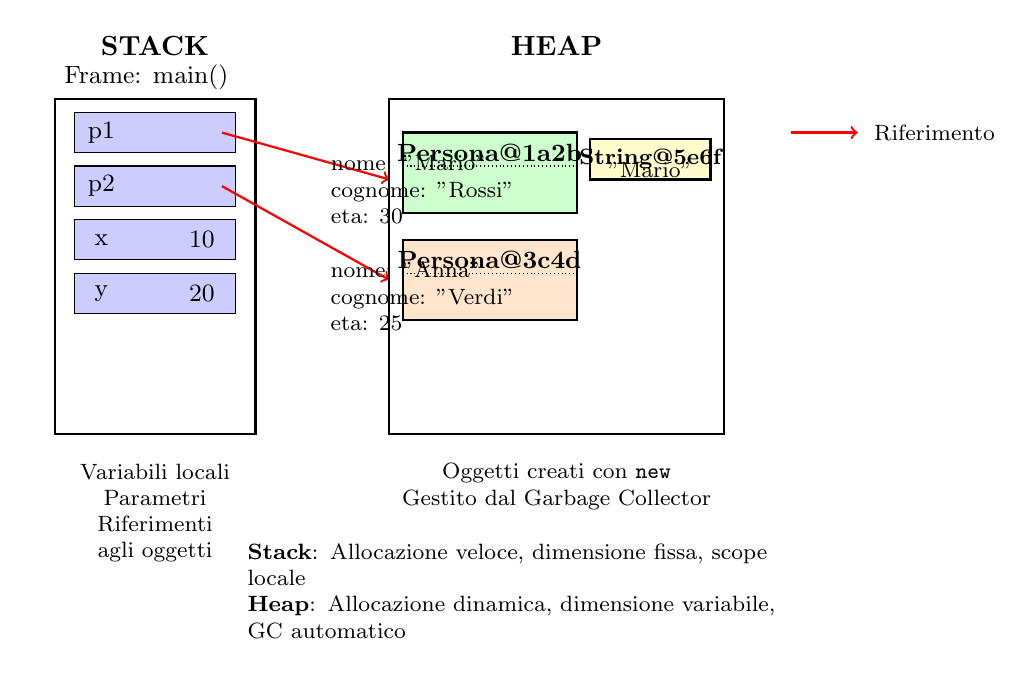
\begin{tikzpicture}[scale=0.85]
    % Stack (sinistra)
    \node[font=\bfseries, above] at (1.5, 5.5) {STACK};
    \draw[thick] (0,0) rectangle (3,5);
    \node[above right, font=\small] at (0,5) {Frame: main()};

    % Variabili locali nello stack
    \draw[fill=blue!20] (0.3,4.2) rectangle (2.7,4.8);
    \node[font=\small] at (0.7,4.5) {p1};
    \draw[->, thick, red] (2.5,4.5) -- (5,3.8);

    \draw[fill=blue!20] (0.3,3.4) rectangle (2.7,4.0);
    \node[font=\small] at (0.7,3.7) {p2};
    \draw[->, thick, red] (2.5,3.7) -- (5,2.3);

    \draw[fill=blue!20] (0.3,2.6) rectangle (2.7,3.2);
    \node[font=\small] at (0.7,2.9) {x};
    \node[font=\small] at (2.2,2.9) {10};

    \draw[fill=blue!20] (0.3,1.8) rectangle (2.7,2.4);
    \node[font=\small] at (0.7,2.1) {y};
    \node[font=\small] at (2.2,2.1) {20};

    % Annotazioni Stack
    \node[below, font=\footnotesize, align=center, text width=3cm] at (1.5,-0.3) {
        Variabili locali\\
        Parametri\\
        Riferimenti agli oggetti
    };

    % Heap (destra)
    \node[font=\bfseries, above] at (7.5, 5.5) {HEAP};
    \draw[thick] (5,0) rectangle (10,5);

    % Oggetto Persona p1
    \draw[fill=green!20, thick] (5.2,3.3) rectangle (7.8,4.5);
    \node[font=\small\bfseries] at (6.5,4.2) {Persona@1a2b};
    \draw[densely dotted] (5.2,4.0) -- (7.8,4.0);
    \node[font=\footnotesize, align=left] at (5.5,3.65) {
        nome: "Mario"\\
        cognome: "Rossi"\\
        eta: 30
    };

    % Oggetto Persona p2
    \draw[fill=orange!20, thick] (5.2,1.7) rectangle (7.8,2.9);
    \node[font=\small\bfseries] at (6.5,2.6) {Persona@3c4d};
    \draw[densely dotted] (5.2,2.4) -- (7.8,2.4);
    \node[font=\footnotesize, align=left] at (5.5,2.05) {
        nome: "Anna"\\
        cognome: "Verdi"\\
        eta: 25
    };

    % Oggetto String (condiviso)
    \draw[fill=yellow!20, thick] (8.0,3.8) rectangle (9.8,4.4);
    \node[font=\footnotesize\bfseries] at (8.9,4.1) {String@5e6f};
    \node[font=\footnotesize] at (8.9,3.95) {"Mario"};

    % Annotazioni Heap
    \node[below, font=\footnotesize, align=center, text width=5cm] at (7.5,-0.3) {
        Oggetti creati con \texttt{new}\\
        Gestito dal Garbage Collector
    };

    % Legenda
    \draw[->, thick, red] (11,4.5) -- (12,4.5);
    \node[right, font=\footnotesize] at (12.1,4.5) {Riferimento};

    % Note esplicative
    \node[below, font=\footnotesize, align=left, text width=7cm] at (7,-1.5) {
        \textbf{Stack}: Allocazione veloce, dimensione fissa, scope locale\\
        \textbf{Heap}: Allocazione dinamica, dimensione variabile, GC automatico
    };
\end{tikzpicture}
\end{center}

\begin{description}
    \item[Stack:] Contiene variabili locali, parametri dei metodi e riferimenti agli oggetti. Lo stack è organizzato per frame (ogni metodo ha il suo frame). Quando un metodo termina, il suo frame viene rimosso.

    \item[Heap:] Contiene gli oggetti effettivi creati con \texttt{new}. Gli oggetti nell'heap possono essere accessibili da più variabili (riferimenti). Il Garbage Collector rimuove automaticamente gli oggetti non più referenziati.

    \item[Riferimenti:] Le variabili di tipo oggetto (\texttt{Persona p1}) contengono riferimenti (indirizzi) agli oggetti nell'heap, non gli oggetti stessi. I tipi primitivi (\texttt{int x}) contengono direttamente il valore.
\end{description}

\begin{tcolorbox}[colback=blue!10, colframe=blue!60, title=Esempio pratico]
\begin{lstlisting}
public static void main(String[] args) {
    // Stack: crea riferimento p1 (null inizialmente)
    Persona p1;

    // Heap: crea oggetto Persona, Stack: p1 punta all'oggetto
    p1 = new Persona("Mario", "Rossi", 30);

    // Stack: crea p2 che punta allo STESSO oggetto di p1
    Persona p2 = p1;

    // Modificando p2, modifichi l'oggetto puntato anche da p1!
    p2.setEta(31);
    System.out.println(p1.getEta());  // Stampa 31!
}
\end{lstlisting}
\end{tcolorbox}

\begin{attenzione}
Quando assegni \texttt{p2 = p1}, stai copiando il \textbf{riferimento}, non l'oggetto! Entrambe le variabili puntano allo stesso oggetto nell'heap. Se vuoi una copia indipendente, devi creare un nuovo oggetto.
\end{attenzione}

\section{Costruttori e Metodi}

Le classi non sono complete senza costruttori per inizializzare gli oggetti e metodi per definirne il comportamento.

\subsection{Costruttori: L'Inizializzazione degli Oggetti}
Un \textbf{costruttore} è un metodo speciale che viene invocato automaticamente quando si crea un nuovo oggetto di una classe usando l'operatore \texttt{new}. Il suo scopo principale è inizializzare lo stato dell'oggetto. Un costruttore deve avere lo \textbf{stesso nome} della classe che sta inizializzando. A differenza dei metodi ordinari, un costruttore non ha un \textbf{tipo di ritorno}, nemmeno \texttt{void}. Se non viene definito alcun costruttore, Java ne fornisce uno \textbf{di default} senza parametri che inizializza semplicemente gli attributi con i valori di default del loro tipo.

\subsubsection{Costruttore con Parametri}
Permette di inizializzare gli attributi con valori specifici al momento della creazione dell'oggetto.

\begin{lstlisting}
public class Persona {
    private String nome;
    private String cognome;
    private int eta;

    // Costruttore con parametri
    public Persona(String nome, String cognome, int eta) {
        this.nome = nome;        // 'this.nome' si riferisce all'attributo della classe
        this.cognome = cognome;  // 'nome' si riferisce al parametro del costruttore
        this.eta = eta;
    }
}
\end{lstlisting}
\texttt{this}: La parola chiave \texttt{this} è un riferimento all'istanza corrente dell'oggetto. È usata per distinguere gli attributi di istanza dai parametri locali che hanno lo stesso nome.

\subsubsection{Costruttori di Default e Completo}
I costruttori permettono di inizializzare gli oggetti della classe.  
Il \textbf{costruttore di default} fornisce valori predefiniti quando non vengono specificate informazioni, mentre il \textbf{costruttore completo} permette di impostare tutti i parametri della classe al momento della creazione dell'oggetto.

\begin{lstlisting}
public class Persona {
    private String nome;
    private String cognome;
    private int eta;

    // Costruttore completo
    public Persona(String nome, String cognome, int eta) {
        this.nome = nome;
        this.cognome = cognome;
        this.eta = eta;
    }

    // Costruttore di default che richiama quello completo
    public Persona() {
        this("Sconosciuto", "Sconosciuto", 0);
    }
}
\end{lstlisting}


\subsection{Metodi: Il Comportamento degli Oggetti}
I \textbf{metodi} sono blocchi di codice che definiscono il comportamento o le azioni che un oggetto può compiere. Possono accedere e modificare lo stato degli attributi dell'oggetto.

\begin{lstlisting}
public class Persona {
    private String nome;
    private String cognome;
    private int eta;

    // Metodo per visualizzare le informazioni
    public void stampaInfo() {
        System.out.println(nome + " " + cognome + ", " + eta + " anni");
    }

    // Metodo per verificare se la persona è maggiorenne
    public boolean isMaggiorenne() {
        return eta >= 18;
    }
}
\end{lstlisting}

\textbf{Esempio di Utilizzo della Classe Persona:}

\begin{lstlisting}
public class TestPersona {
    public static void main(String[] args) {
        // Creazione di oggetti usando diversi costruttori
        Persona p1 = new Persona("Mario", "Rossi", 25);
        Persona p2 = new Persona(); // Usa costruttore di default
        Persona p3 = new Persona("Laura", "Bianchi", 17);

        // Invocazione di metodi sugli oggetti
        p1.stampaInfo(); // Output: Mario Rossi, 25 anni

        if (p3.isMaggiorenne()) {
            // System.out.println(p3.nome + " è maggiorenne."); // Errore: nome è private
             System.out.println("Laura è maggiorenne."); // Versione corretta
        } else {
            // System.out.println(p3.cognome + " è minorenne."); // Errore: cognome è private
            System.out.println("Laura è minorenne."); // Versione corretta
        }
        // Nota: Qui si incorrerebbe in un errore di compilazione
        // perché nome e cognome sono privati. Vedremo come accedere
        // ad essi tramite getter e setter.
    }
}
\end{lstlisting}

\subsection{Overloading dei Metodi (Sovraccarico)}
L'\textbf{overloading} permette di definire più metodi con lo stesso nome all'interno della stessa classe, purché abbiano una \textbf{firma diversa}. La firma di un metodo è determinata dal suo nome e dalla lista dei tipi dei parametri, e dal loro ordine. Il tipo di ritorno non è parte della firma per l'overloading.

\subsubsection{Regole dell'Overloading}
L'overloading segue regole precise per distinguere diversi metodi con lo stesso nome. Innanzitutto, i metodi devono avere lo stesso nome. Tuttavia, la loro lista di parametri deve essere diversa, variando nel numero dei parametri, nel tipo dei parametri, o nell'ordine dei tipi. È importante notare che il tipo di ritorno può essere lo stesso o diverso senza influenzare il riconoscimento dell'overloading: il compilatore identifica il metodo corretto basandosi solo sulla firma (nome e parametri), non sul tipo di ritorno.

\subsubsection{Esempio: Overloading di Costruttori nella Classe Persona}
Abbiamo già visto questo nella classe \texttt{Persona} con il costruttore con parametri e quello di default. Possiamo aggiungere un terzo costruttore:

\begin{lstlisting}
public class Persona {
    private String nome;
    private String cognome;
    private int eta;

    // 1. Costruttore con 3 parametri
    public Persona(String nome, String cognome, int eta) {
        this.nome = nome;
        this.cognome = cognome;
        this.eta = eta;
    }

    // 2. Costruttore senza parametri (overloading)
    public Persona() {
        this("Sconosciuto", "Sconosciuto", 0); // Chiama il costruttore #1
    }

    // 3. Costruttore con 2 parametri (overloading)
    public Persona(String nome, String cognome) {
        this(nome, cognome, 0); // Chiama il costruttore #1, impostando età a 0
    }
}
\end{lstlisting}
\texttt{this()}: Un costruttore può chiamare un altro costruttore della stessa classe usando \texttt{this()}. Deve essere la prima istruzione del costruttore chiamante.

\subsubsection{Esempio: Overloading di un Metodo \texttt{calcola}}

\begin{lstlisting}
public class Calcolatrice {

    // Somma due interi
    public int calcola(int a, int b) {
        return a + b;
    }

    // Somma tre interi (overloading: numero di parametri diverso)
    public int calcola(int a, int b, int c) {
        return a + b + c;
    }

    // Somma due double (overloading: tipo di parametri diverso)
    public double calcola(double a, double b) {
        return a + b;
    }

    // Esempio di utilizzo
    public static void main(String[] args) {
        Calcolatrice calc = new Calcolatrice();

        System.out.println(calc.calcola(5, 3));         // Chiama calcola(int, int)
        System.out.println(calc.calcola(5, 3, 2));      // Chiama calcola(int, int, int)
        System.out.println(calc.calcola(5.5, 3.2));     // Chiama calcola(double, double)
    }
}
\end{lstlisting}

\section{UML: Rappresentare Classi e Relazioni}

I diagrammi UML (Unified Modeling Language) sono uno strumento standard per visualizzare, specificare, costruire e documentare gli artefatti di un sistema software. I diagrammi di classe UML sono particolarmente utili per mostrare le classi, i loro attributi, i loro metodi e le relazioni tra di esse.

\subsection{Sintassi Base del Diagramma di Classe UML}
Un rettangolo diviso in tre sezioni rappresenta una classe in UML. La \textbf{sezione superiore} contiene il nome della classe. La \textbf{sezione centrale} elenca gli attributi della classe con il loro tipo. La \textbf{sezione inferiore} racchiude i metodi della classe con la loro firma (parametri e tipo di ritorno).

\textbf{Visibilità (Modificatori di Accesso) in UML:} I modificatori di accesso in UML sono rappresentati con simboli speciali per indicare il livello di visibilità. Il simbolo \texttt{+ } (più) rappresenta \textbf{public}, accessibile da qualsiasi altra classe. Il simbolo \texttt{- } (meno) rappresenta \textbf{private}, accessibile solo all'interno della classe stessa. Il simbolo \texttt{\# } (cancelletto) rappresenta \textbf{protected}, accessibile all'interno della classe, nelle sottoclassi e nello stesso package. Il simbolo \texttt{\~{}} (tilde) rappresenta \textbf{package-private} o \textbf{default}, accessibile solo dalle classi dello stesso package.

\subsubsection{Esempio: Diagramma UML della Classe \texttt{Persona}}

Rappresentiamo la nostra classe \texttt{Persona} con i costruttori e i metodi visti finora.
%TODO: GENERA TU L'UML

\section{Array di Oggetti}

Gli array di oggetti ci permettono di gestire collezioni di istanze della stessa classe in modo efficiente. A differenza degli array di tipi primitivi, un array di oggetti contiene \textbf{riferimenti} agli oggetti, non gli oggetti stessi.

\subsection{Dichiarazione e Inizializzazione di Array di Oggetti}

\begin{lstlisting}
public class Studente {
    private String matricola;
    private String nome;
    private double media;

    public Studente(String matricola, String nome, double media) {
        this.matricola = matricola;
        this.nome = nome;
        this.media = media;
    }

    // Metodi getter (per ora, per accesso agli attributi)
    public String getMatricola() { return matricola; }
    public String getNome() { return nome; }
    public double getMedia() { return media; }

    public boolean isPromosso() {
        return media >= 6.0;
    }

    // Metodo toString per una rappresentazione testuale dell'oggetto
    @Override
    public String toString() {
        return "Studente [Matricola=" + matricola + ", Nome=" + nome + ", Media=" + media + "]";
    }
}
\end{lstlisting}

\textbf{Creazione e Utilizzo di un Array di \texttt{Studente}:}

\begin{lstlisting}
public class GestioneClasse {
    public static void main(String[] args) {
        // Dichiarazione e creazione di un array di 3 riferimenti a Studente
        Studente[] classe = new Studente[3];

        // Inizializzazione di ogni elemento dell'array con un nuovo oggetto Studente
        classe[0] = new Studente("A001", "Alice Rossi", 7.8);
        classe[1] = new Studente("A002", "Bob Bianchi", 5.2);
        classe[2] = new Studente("A003", "Carlo Verdi", 8.5);

        System.out.println("--- Elenco Studenti ---");
        // Iterazione con for tradizionale
        for (int i = 0; i < classe.length; i++) {
            System.out.println(classe[i].toString()); // Chiama il metodo toString() di ogni oggetto
        }

        System.out.println("\n--- Studenti Promossi ---");
        // Iterazione con for-each (più concisa per percorrere collezioni)
        for (Studente s : classe) {
            if (s.isPromosso()) {
                System.out.println(s.getNome() + " è promosso!");
            }
        }
    }
}
\end{lstlisting}

\textbf{Punti Chiave:} Quando si dichiara `Studente[] classe = new Studente[3];`, si crea un array di tre \emph{riferimenti} a `Studente`, ognuno inizializzato a `null`. Non crea automaticamente gli oggetti. È quindi necessario creare esplicitamente un oggetto `Studente` per ogni posizione dell'array tramite `classe[0] = new Studente(...)`, altrimenti tenteremo di accedere a un oggetto `null`, causando una `NullPointerException`. Una volta che gli oggetti sono stati creati, possiamo accedere ai loro attributi e invocare i loro metodi utilizzando la notazione `classe[i].metodo()` per l'accesso tramite indice, oppure `s.metodo()` quando iteriamo con un ciclo for-each assegnando ogni elemento a una variabile come `s`.

\section{Metodi Statici, Metodo \texttt{toString()}, Getter e Setter}

Questa sezione approfondisce alcuni metodi e convenzioni importanti per la gestione delle classi.

\subsection{Metodi Statici e Attributi Statici}
Gli elementi \textbf{statici} (attributi o metodi) appartengono alla classe stessa, non a una specifica istanza (oggetto) della classe. Vengono caricati in memoria una sola volta quando la classe viene caricata e sono condivisi da tutte le istanze della classe. Gli elementi statici si invocano direttamente sulla classe, non sull'oggetto, utilizzando la sintassi `NomeClasse.metodoStatico()` oppure `NomeClasse.attributoStatico`. Una limitazione importante è che i metodi statici possono accedere solo ad altri membri statici della classe. Non possono accedere a membri non statici (di istanza) perché questi ultimi esistono solo in relazione a uno specifico oggetto, mentre i metodi statici non hanno un contesto di istanza.

\subsubsection{Esempio: Classe \texttt{Contatore} con Membri Statici}

\begin{lstlisting}
public class Contatore {
    private static int conteggioGlobale = 0; // Attributo statico, condiviso da tutte le istanze
    private int idIstanza; // Attributo di istanza

    public Contatore() {
        conteggioGlobale++; // Incrementa il contatore globale ogni volta che un oggetto viene creato
        this.idIstanza = conteggioGlobale; // Assegna un ID univoco all'istanza
    }

    // Metodo statico: restituisce il conteggio totale degli oggetti creati
    public static int getConteggioGlobale() {
        return conteggioGlobale;
    }

    // Metodo di istanza: restituisce l'ID di questa specifica istanza
    public int getIdIstanza() {
        return idIstanza;
    }

    public static void main(String[] args) {
        System.out.println("Contatore globale iniziale: " + Contatore.getConteggioGlobale()); // 0

        Contatore c1 = new Contatore();
        Contatore c2 = new Contatore();
        Contatore c3 = new Contatore();

        System.out.println("ID c1: " + c1.getIdIstanza()); // 1
        System.out.println("ID c2: " + c2.getIdIstanza()); // 2
        System.out.println("ID c3: " + c3.getIdIstanza()); // 3

        System.out.println("Contatore globale finale: " + Contatore.getConteggioGlobale()); // 3
    }
}
\end{lstlisting}

\subsection{Il Metodo \texttt{toString()}}
Il metodo \texttt{toString()} è ereditato da tutte le classi Java dalla classe base \texttt{Object}. Il suo scopo è fornire una rappresentazione testuale dell'oggetto. È buona pratica fare l'override di questo metodo per restituire una stringa significativa per la nostra classe.

\begin{lstlisting}
public class Prodotto {
    private String codice;
    private String descrizione;
    private double prezzo;

    public Prodotto(String codice, String descrizione, double prezzo) {
        this.codice = codice;
        this.descrizione = descrizione;
        this.prezzo = prezzo;
    }

    @Override // L'annotazione @Override è consigliata
    public String toString() {
        return "Prodotto [Codice=" + codice + ", Descrizione=" + descrizione + ", Prezzo=" + prezzo + "]";
    }

    public static void main(String[] args) {
        Prodotto p = new Prodotto("P001", "Laptop", 1200.0);
        System.out.println(p); // Chiama automaticamente p.toString()
        System.out.println("Dettagli: " + p); // Anche la concatenazione chiama toString()
    }
}
\end{lstlisting}

\subsection{Getter (Accessors) e Setter (Mutators)}
I \textbf{getter} e i \textbf{setter} sono metodi pubblici utilizzati per accedere e modificare gli attributi privati di una classe. Sono fondamentali per l'incapsulamento, poiché permettono di controllare come i dati vengono letti e scritti. I \textbf{getter} sono metodi che restituiscono il valore di un attributo seguendo la convenzione `getNomeAttributo()`, oppure `isNomeAttributo()` per gli attributi di tipo booleano. I \textbf{setter} sono metodi che impostano il valore di un attributo seguendo la convenzione `setNomeAttributo(tipo valore)`. Un aspetto importante è che nei setter è possibile includere logica di validazione per assicurare che solo valori appropriati vengano assegnati agli attributi.

\subsubsection{Esempio: Getter e Setter nella Classe \texttt{Studente}}

Aggiorniamo la classe \texttt{Studente} con getter e setter completi.

\begin{lstlisting}
public class Studente {
    private String matricola;
    private String nome;
    private double media;

    public Studente(String matricola, String nome, double media) {
        this.matricola = matricola;
        this.nome = nome;
        this.media = media;
    }

    // Getter
    public String getMatricola() {
        return matricola;
    }

    public String getNome() {
        return nome;
    }

    public double getMedia() {
        return media;
    }

    // Setter (con validazione per la media)
    public void setMatricola(String matricola) {
        this.matricola = matricola;
    }

    public void setNome(String nome) {
        this.nome = nome;
    }

    public void setMedia(double media) {
        if (media >= 0.0 && media <= 10.0) { // Validazione
            this.media = media;
        } else {
            System.out.println("Errore: Media non valida (deve essere tra 0 e 10)");
        }
    }

    public boolean isPromosso() {
        return media >= 6.0;
    }

    @Override
    public String toString() {
        return "Studente [Matricola=" + matricola + ", Nome=" + nome + ", Media=" + media + "]";
    }

    public static void main(String[] args) {
        Studente s1 = new Studente("B001", "Giulia Rossi", 7.0);
        System.out.println(s1.getNome() + " ha media: " + s1.getMedia()); // Accedo tramite getter

        s1.setMedia(9.5); // Modifico tramite setter
        System.out.println(s1.getNome() + " nuova media: " + s1.getMedia());

        s1.setMedia(12.0); // Tentativo di impostare una media non valida
        System.out.println(s1.getNome() + " media dopo tentativo non valido: " + s1.getMedia()); // La media rimane 9.5
    }
}
\end{lstlisting}
Fino a questo punto, abbiamo gestito gli attributi della classe come `private` e i metodi (costruttori, di utilità, getter e setter) come `public`. Questa è una best practice per garantire un forte incapsulamento.

\section{Ereditarietà}

L'\textbf{ereditarietà} è un pilastro fondamentale dell'OOP che permette di creare una gerarchia di classi. Una classe (sottoclasse o classe derivata) può ereditare attributi e metodi da un'altra classe (superclasse o classe base), stabilendo una relazione "è un" (is-a).

\subsection{La Parola Chiave \texttt{extends}}
In Java, l'ereditarietà si implementa con la parola chiave \texttt{extends}.

\begin{lstlisting}
// Superclasse
public class Veicolo {
    protected String targa;
    protected int annoImmatricolazione;
    protected double velocitaMassima;

    public Veicolo(String targa, int anno, double vMax) {
        this.targa = targa;
        this.annoImmatricolazione = anno;
        this.velocitaMassima = vMax;
    }

    public void mostraInfo() {
        System.out.println("Veicolo targa: " + targa);
        System.out.println("Anno: " + annoImmatricolazione);
        System.out.println("V.max: " + velocitaMassima + " km/h");
    }

    public double calcolaBollo() {
        return 100.0; // Calcolo base del bollo
    }
}
\end{lstlisting}

\textbf{Modificatore \texttt{protected}}: Permette agli attributi di essere accessibili all'interno della classe stessa e in tutte le sue sottoclassi, ma non da classi esterne non correlate. Questo è ideale per l'ereditarietà.

\subsubsection{Diagramma UML di Ereditarietà}

Questo diagramma mostra la relazione "è un" tra \texttt{Veicolo} (superclasse) e \texttt{Auto}, \texttt{Moto} (sottoclassi).
%TODO: GENERA TU L'UML

\subsection{Sottoclasse \texttt{Auto}}

\begin{lstlisting}
public class Auto extends Veicolo {
    private int numeroPosti;
    private String alimentazione;

    public Auto(String targa, int anno, double vMax, int posti, String alimentazione) {
        super(targa, anno, vMax); // Chiama il costruttore della superclasse Veicolo
        this.numeroPosti = posti;
        this.alimentazione = alimentazione;
    }

    // Override del metodo della superclasse per aggiungere informazioni specifiche
    @Override
    public void mostraInfo() {
        super.mostraInfo(); // Chiama il metodo mostraInfo() di Veicolo
        System.out.println("Posti: " + numeroPosti);
        System.out.println("Alimentazione: " + alimentazione);
    }

    // Override del metodo calcolaBollo() per implementare una logica specifica per le auto
    @Override
    public double calcolaBollo() {
        double bolloBase = super.calcolaBollo(); // Ottiene il bollo base dalla superclasse
        if (alimentazione.equalsIgnoreCase("elettrica")) {
            return bolloBase * 0.5; // Auto elettriche hanno sconto del 50%
        }
        return bolloBase;
    }

    // Metodo specifico della sottoclasse Auto
    public boolean isFamiliare() {
        return numeroPosti >= 5;
    }
}
\end{lstlisting}

\textbf{Parola chiave \texttt{super}}:
\begin{itemize}
    \item `super(...)`: Deve essere la prima istruzione in un costruttore di sottoclasse per invocare un costruttore della superclasse.
    \item `super.metodo()`: Permette di invocare un metodo della superclasse, utile quando si vuole estendere il comportamento piuttosto che sostituirlo completamente.
\end{itemize}

\subsection{Override dei Metodi (Sovrascrittura)}
L'\textbf{override} è il meccanismo attraverso il quale una sottoclasse fornisce la propria implementazione di un metodo che è già stato definito nella sua superclasse.

\subsubsection{Regole dell'Override}
\begin{itemize}
    \item Stessa firma del metodo (nome, numero, tipo e ordine dei parametri).
    \item Il tipo di ritorno deve essere uguale o un sottotipo (covariante).
    \item Il modificatore di accesso non può essere più restrittivo di quello della superclasse.
    \item L'annotazione `@Override` è facoltativa ma altamente consigliata per prevenire errori.
\end{itemize}

\subsubsection{Differenze tra Overload e Override}
\begin{center}
\begin{tabular}{|p{5.5cm}|p{5.5cm}|}
\hline
\textbf{OVERLOAD} (Sovraccarico) & \textbf{OVERRIDE} (Sovrascrittura) \\
\hline
Stessa classe & Superclasse e sottoclasse \\
\hline
Stesso nome, parametri diversi & Stessa firma (nome e parametri) \\
\hline
Risoluzione a tempo di compilazione (binding statico) & Risoluzione a tempo di esecuzione (binding dinamico) \\
\hline
Aumenta la flessibilità & Specializza il comportamento \\
\hline
Non richiede ereditarietà & Richiede ereditarietà \\
\hline
\end{tabular}
\end{center}

\subsection{Sottoclasse \texttt{Moto}}

\begin{lstlisting}
public class Moto extends Veicolo {
    private int cilindrata;
    private boolean hasBauletto;

    public Moto(String targa, int anno, double vMax, int cilindrata, boolean bauletto) {
        super(targa, anno, vMax);
        this.cilindrata = cilindrata;
        this.hasBauletto = bauletto;
    }

    @Override
    public void mostraInfo() {
        super.mostraInfo();
        System.out.println("Cilindrata: " + cilindrata + " cc");
        System.out.println("Bauletto: " + (hasBauletto ? "Sì" : "No"));
    }

    @Override
    public double calcolaBollo() {
        if (cilindrata <= 125) {
            return 50.0;
        } else if (cilindrata <= 500) {
            return 80.0;
        } else {
            return 120.0;
        }
    }
}
\end{lstlisting}

Qui il metodo `calcolaBollo()` della classe `Moto` sostituisce completamente la logica della superclasse, dimostrando un altro modo di utilizzare l'override.

\section{Polimorfismo}

Il \textbf{polimorfismo} (dal greco "molte forme") è la capacità di un'entità di assumere forme diverse. In OOP, significa che un riferimento a una superclasse può riferirsi a oggetti di qualsiasi sua sottoclasse. Questo permette di scrivere codice più generale e flessibile.

\subsection{Esempio di Polimorfismo con i Veicoli}

\begin{lstlisting}
public class GestioneParcoVeicoli {
    public static void main(String[] args) {
        // Un array di riferimenti di tipo Veicolo può contenere oggetti Auto e Moto
        Veicolo[] parcoVeicoli = new Veicolo[4];

        parcoVeicoli[0] = new Auto("AB123CD", 2020, 180.0, 5, "benzina");
        parcoVeicoli[1] = new Moto("EF456GH", 2021, 200.0, 600, true);
        parcoVeicoli[2] = new Auto("IJ789KL", 2023, 150.0, 4, "elettrica");
        parcoVeicoli[3] = new Moto("MN012OP", 2019, 160.0, 125, false);

        System.out.println("=== Dettagli e Bolli dei Veicoli ===\n");

        double totaleBolli = 0;
        for (Veicolo v : parcoVeicoli) {
            v.mostraInfo(); // Chiama la versione specifica (Auto o Moto) a runtime
            double bollo = v.calcolaBollo(); // Chiama la versione specifica (Auto o Moto) a runtime
            System.out.println("Bollo da pagare: " + bollo + " euro");
            totaleBolli += bollo;
            System.out.println("--------------------");
        }

        System.out.println("\nTotale complessivo bolli: " + totaleBolli + " euro");

        // Uso di instanceof per distinguere i tipi reali (da usare con moderazione)
        System.out.println("\n--- Conteggio Veicoli ---");
        int autoCount = 0;
        int motoCount = 0;
        for (Veicolo v : parcoVeicoli) {
            if (v instanceof Auto) {
                autoCount++;
            } else if (v instanceof Moto) {
                motoCount++;
            }
        }
        System.out.println("Numero di Auto: " + autoCount);
        System.out.println("Numero di Moto: " + motoCount);
    }
}
\end{lstlisting}

\textbf{Binding Dinamico (Late Binding)}: Quando un metodo sovrascritto viene chiamato su un riferimento di superclasse che punta a un oggetto di sottoclasse, la JVM determina a runtime quale versione del metodo deve essere eseguita, basandosi sul tipo effettivo dell'oggetto e non sul tipo del riferimento. Questo è il cuore del polimorfismo.

\section{Package in Java}

I \textbf{package} sono un meccanismo di raggruppamento per le classi, le interfacce e le altre entità Java. Servono a organizzare il codice in modo logico e gerarchico, evitando conflitti di nomi e controllando l'accesso. Possiamo pensarli come a delle cartelle all'interno del file system per i nostri file \texttt{.java} e \texttt{.class}.

\subsection{Vantaggi dei Package}
I package offrono diversi benefici importanti nell'organizzazione del codice. Primo, permettono l'\textbf{organizzazione} del progetto raggruppando classi correlate, rendendo il codice più gestibile e comprensibile in progetti di grandi dimensioni. Secondo, consentono la \textbf{prevenzione di conflitti di nomi}: due classi con lo stesso nome possono coesistere in package diversi, come \texttt{java.util.Date} e \texttt{java.sql.Date} che sono due classi completamente diverse. Terzo, i package forniscono un \textbf{controllo degli accessi} tramite il livello di visibilità \textit{package-private}, che permette alle classi dello stesso package di accedere ai membri dichiarati con questo modificatore, ma non alle classi esterne al package.

\subsection{Dichiarazione e Naming Convention}
La dichiarazione del package deve essere la \textbf{prima istruzione} non commento in un file sorgente Java.
\begin{lstlisting}
package it.scuola.gestionale.modelli;

public class Studente {
    // ...
}
\end{lstlisting}
\textbf{Naming Convention}: I nomi dei package seguono la convenzione del dominio internet inverso, tutto in minuscolo e separato da punti.

Esempio: \texttt{it.edu.miosito.nomeprogetto.modulo}.

\subsection{Struttura delle Directory}
La struttura delle directory del tuo progetto deve rispecchiare esattamente la gerarchia dei package. Se una classe è in \texttt{package it.scuola.gestionale.modelli;}, il suo file \texttt{.java} deve trovarsi in \texttt{project\_root/it/scuola/gestionale/modelli/}.

%TODO: GENERA TU L'UML
\subsection{L'istruzione \texttt{import}}
Per utilizzare una classe di un altro package senza dover specificare il suo \textit{fully qualified name} (nome completo del package + nome della classe), è necessario importarla.

Utilizziamo la direttiva \texttt{import} per questo scopo.

\begin{lstlisting}
package it.scuola.gestionale.applicazione;

// Importa una singola classe
import it.scuola.gestionale.modelli.Studente;
// Importa tutte le classi del package java.util (ma non i suoi sotto-package)
import java.util.ArrayList;

public class MainApp {
    public static void main(String[] args) {
        Studente s = new Studente("C001", "Luca Neri", 6.8);
        ArrayList<Studente> listaStudenti = new ArrayList<>();
        listaStudenti.add(s);
        System.out.println(listaStudenti);
    }
}
\end{lstlisting}

\textbf{Import Statico}: Permette di importare membri statici (metodi o campi) di una classe, consentendone l'uso diretto senza prefisso.
\begin{lstlisting}
import static java.lang.Math.*; // Importa tutti i membri statici della classe Math

public class Calcoli {
    public static void main(String[] args) {
        double raggio = 2.0;
        double area = PI * pow(raggio, 2); // Uso PI e pow() direttamente
        System.out.println("Area: " + area);
    }
}
\end{lstlisting}

\subsection{Package Predefiniti di Java}
Java fornisce una ricca libreria standard organizzata in numerosi package. Il package \texttt{java.lang} contiene classi fondamentali per la programmazione Java come \texttt{String}, \texttt{Math}, \texttt{System}, ed è speciale perché viene \textbf{importato automaticamente} senza necessità di dichiarare import espliciti. Il package \texttt{java.util} fornisce classi di utilità e strutture dati come \texttt{ArrayList}, \texttt{HashMap}, \texttt{Scanner}, che sono essenziali per la gestione di collezioni e utilità varie. Il package \texttt{java.io} contiene le classi per input e output, permettendo di lavorare con file e stream, come \texttt{File}, \texttt{BufferedReader}, \texttt{FileWriter}. Infine, il package \texttt{java.net} offre le classi necessarie per la programmazione di rete, consentendo la creazione di applicazioni client-server e la comunicazione su internet.

\section{Riepilogo}

In questo capitolo abbiamo gettato le basi della programmazione orientata agli oggetti in Java.

Abbiamo esplorato:
\begin{itemize}
    \item I \textbf{pilastri dell'OOP}: Astrazione, Incapsulamento, Ereditarietà, Polimorfismo.
    \item La creazione di \textbf{classi e oggetti}: attributi, costruttori e metodi.
    \item L'\textbf{overloading} per fornire metodi con lo stesso nome ma firme diverse.
    \item L'uso dei \textbf{diagrammi UML} per modellare le classi.
    \item La gestione di \textbf{collezioni di oggetti} tramite array.
    \item I \textbf{membri statici} che appartengono alla classe, non all'istanza.
    \item L'importanza del metodo \textbf{\texttt{toString()}} e dei \textbf{getter/setter} per l'incapsulamento.
    \item L'\textbf{ereditarietà} con \texttt{extends} e \texttt{super} per riuso e specializzazione.
    \item L'\textbf{override} per ridefinire il comportamento nelle sottoclassi.
    \item Il \textbf{polimorfismo} e il binding dinamico per codice flessibile.
    \item L'organizzazione del codice in \textbf{package} per modularità e gestione dei nomi.
\end{itemize}

Questi concetti sono interconnessi e fondamentali per scrivere codice Java efficace, manutenibile e scalabile.


%TODO: Ristruttura il capitolo con questo ordine: Caratteristiche della OOP e del java, Classi, oggetti e attributi; costrutturi e metodi (anche con overloading); UML; array di oggetti;
%Metodi static, metodo toString(); getter e setter  <- fino a qui public i metodi e private gli attributi
%ereditarietà e polimorfismo